\appendix
\chapter{Flow Diagram of Point Cloud Processing}
Below is a flow diagram showing the movement of objects through the process. The primary processes as described in Results and Method are Normal Computation, Segmentation, Segment Selection, Boundary Creation, Extrusion and creation of the Boundary representation. This Flow diagram aims to show how these processes interact with each other to make the understanding of the Method and Results sections easier.

Every process has input objects, these objects are never changed. This means that if a process outputs an object with the same name this object is unchanged in the process.

\begin{figure}[p]
\centering
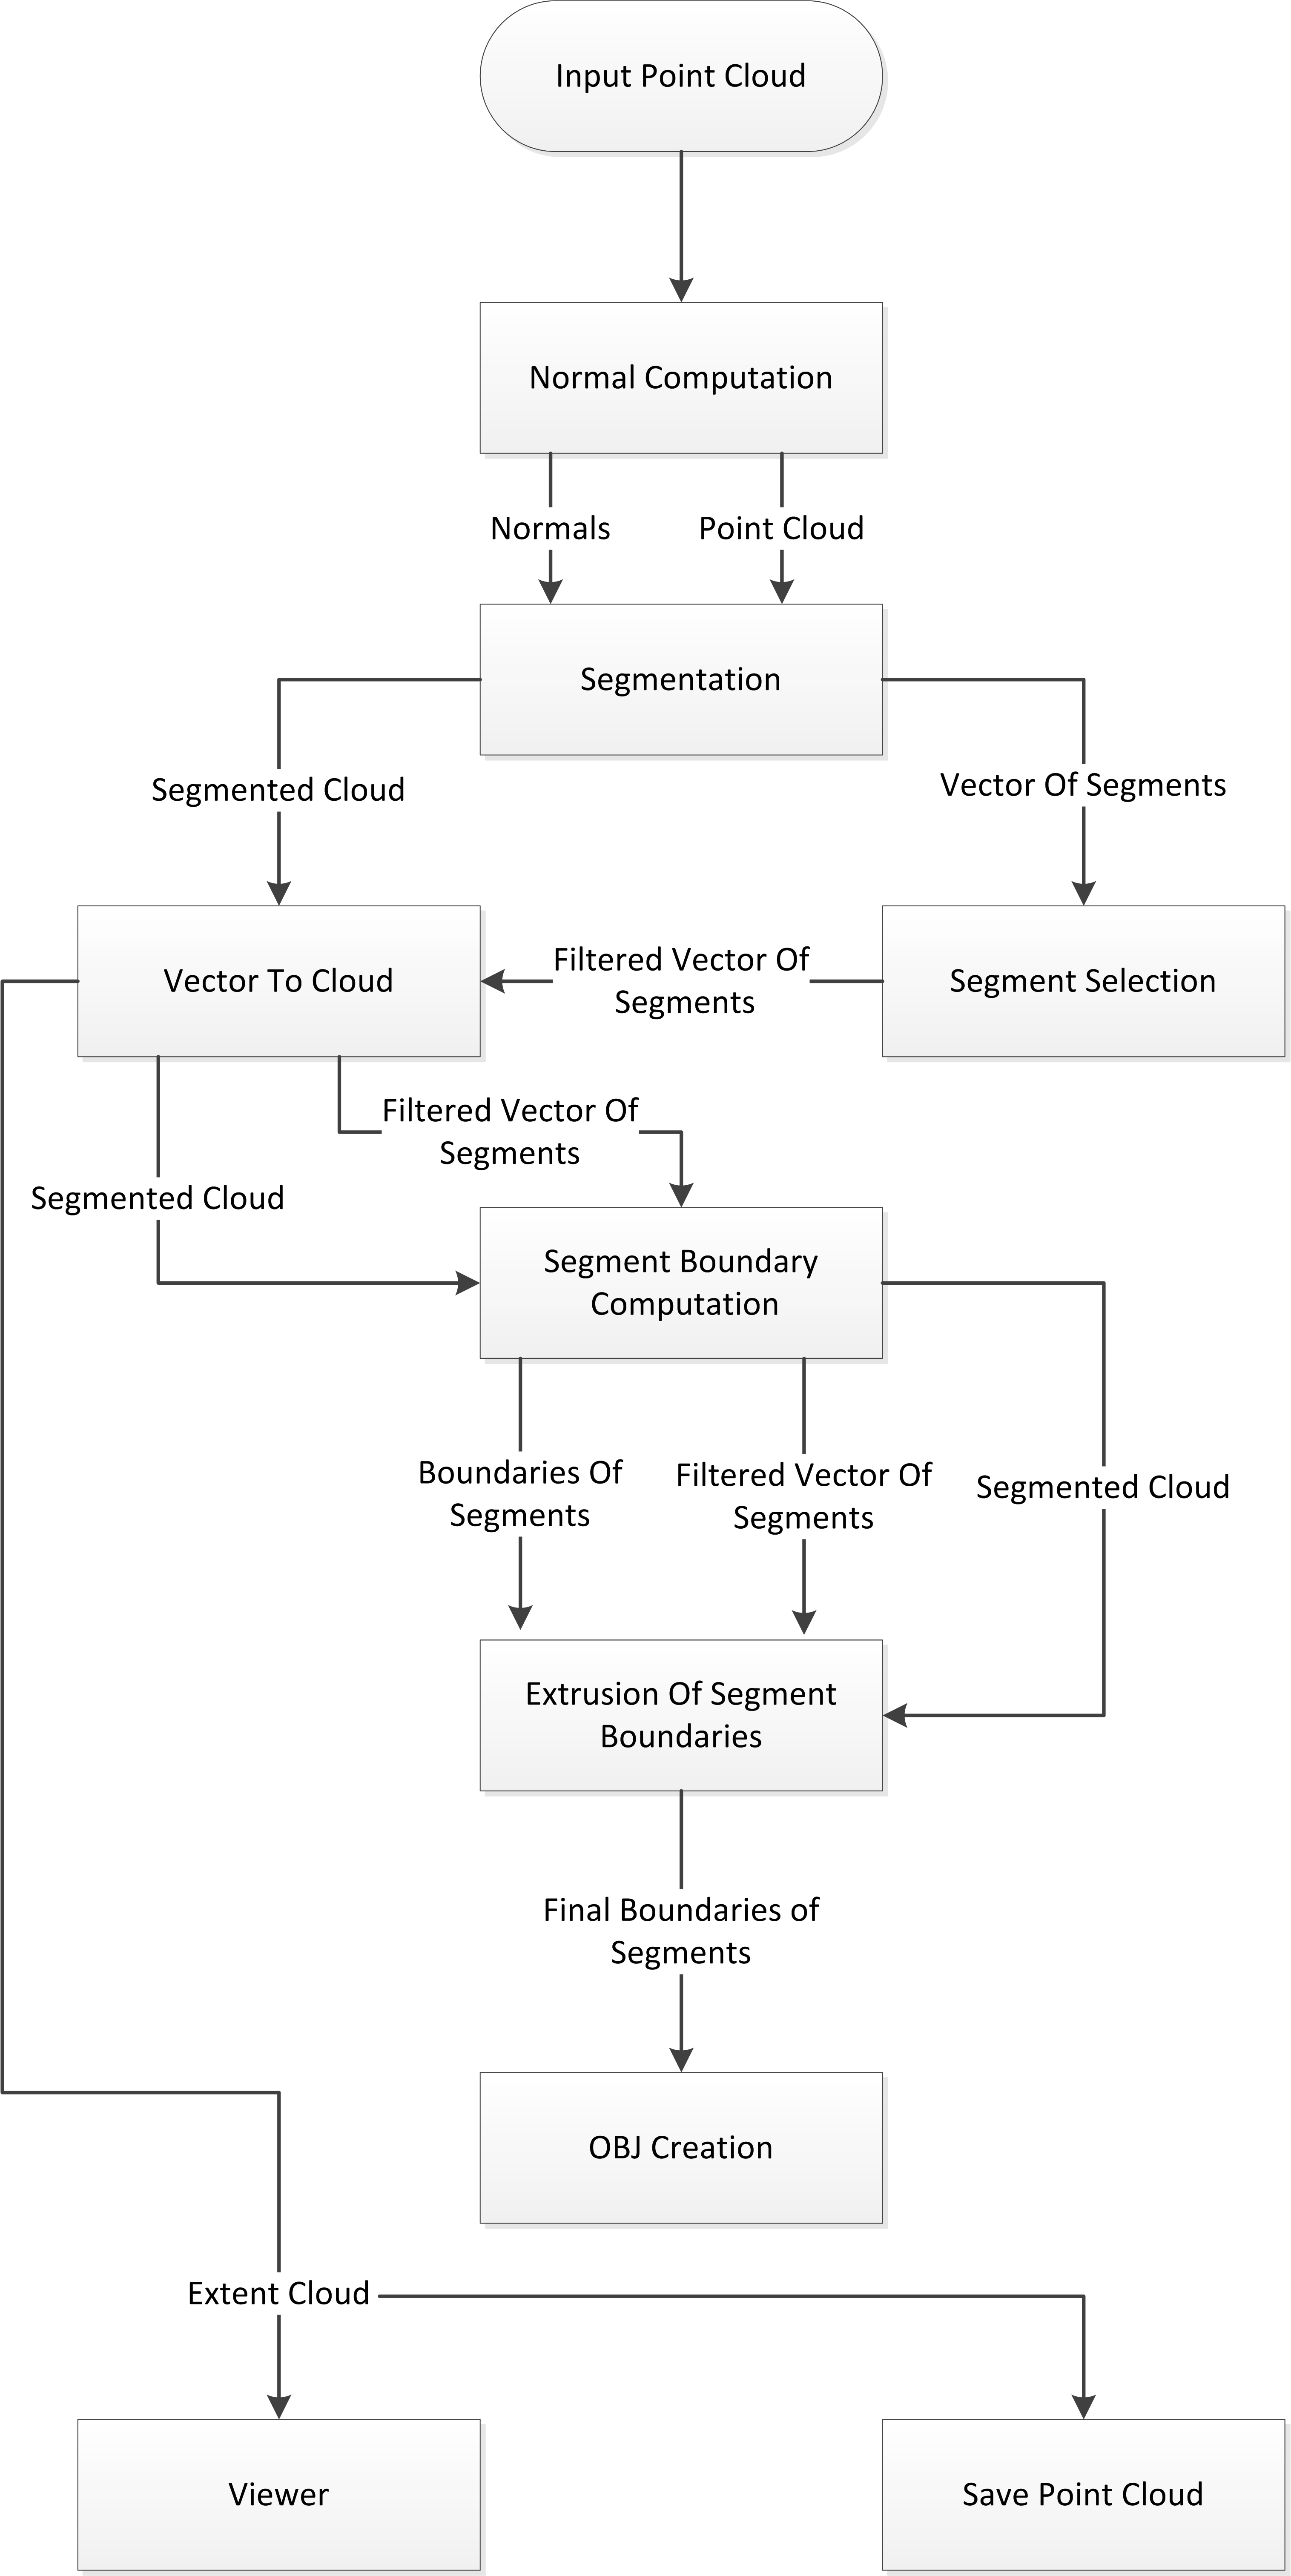
\includegraphics[width=0.7\linewidth]{Includes/images/FlowDiagram}
\caption{Flow Diagram Showing the Movement of Objects Through the Process}
\label{fig:FlowDiagram}
\end{figure}



\chapter{GTL Full Results}
\label{GTL Results}
This whole report is done with a single point cloud to make distinguishing the differences from the steps easier and clearer. The figures that follow are from a different point cloud and show the same process.

These have been added to show the results of processing a different point cloud.

\begin{figure}[H]
\centering
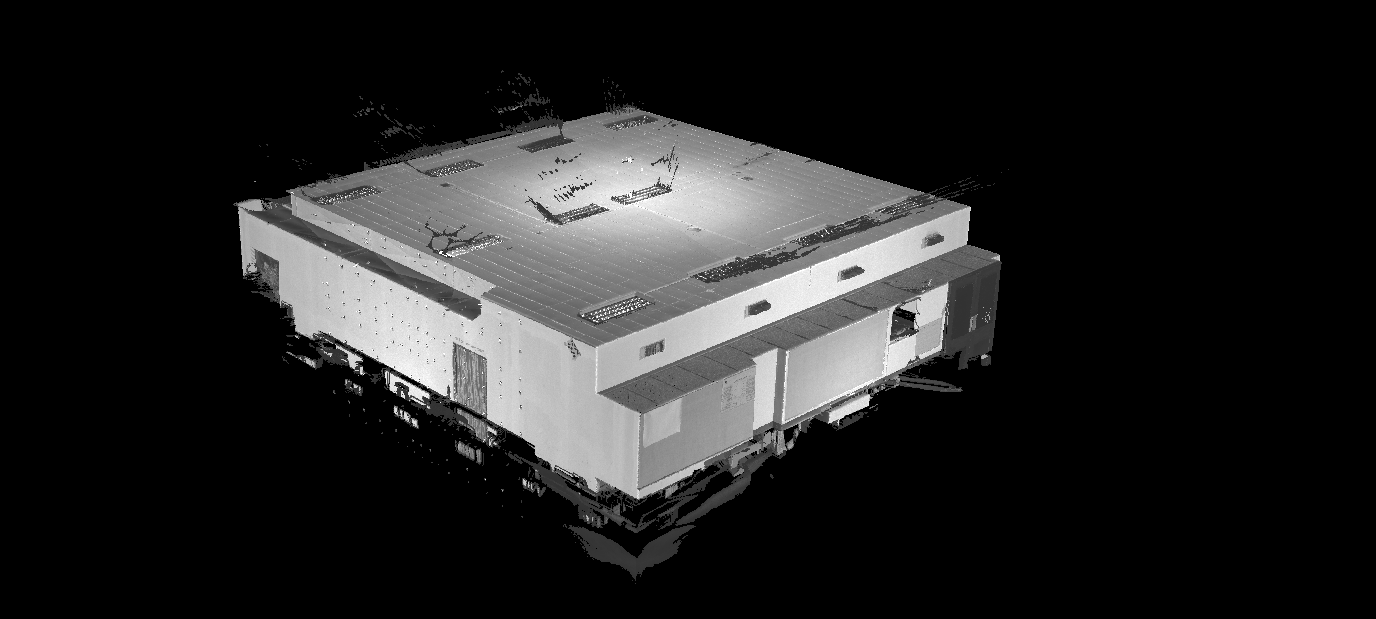
\includegraphics[width=1\linewidth]{Includes/images/Appendix/Before}
\caption{Original Point Cloud}
\label{fig:Before}
\end{figure}

\begin{figure}[H]
\centering
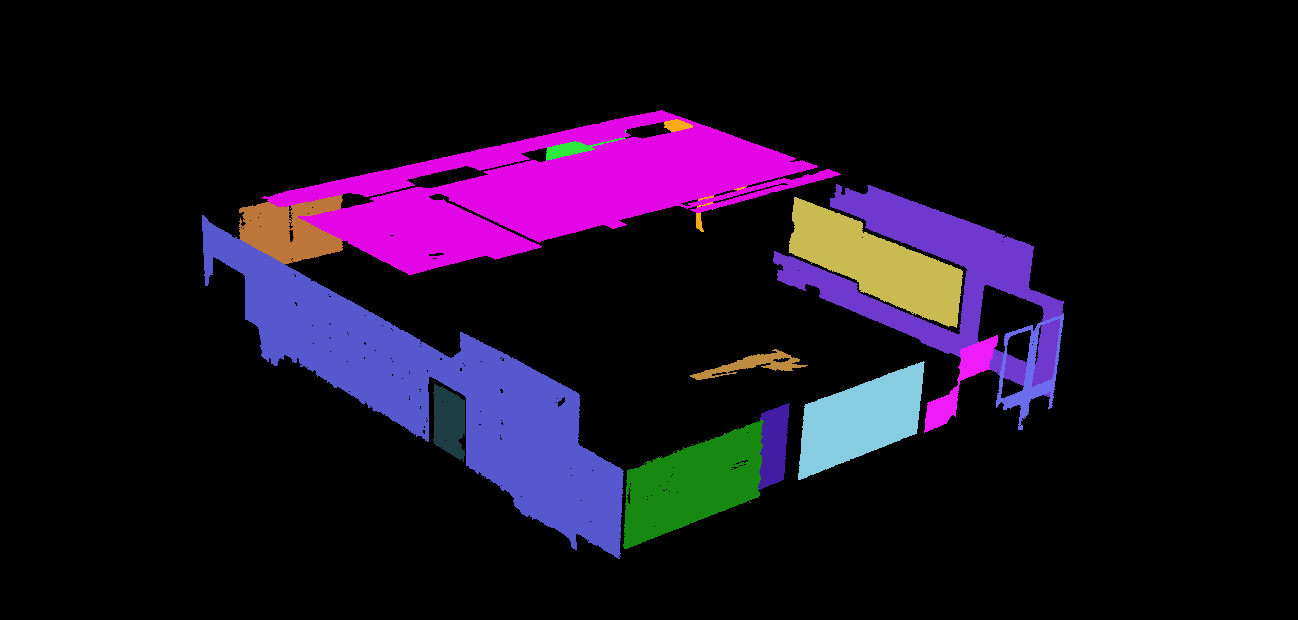
\includegraphics[width=1\linewidth]{Includes/images/Appendix/GTL-Full-seg}
\caption{Point Cloud After Segmentation and Segment Selection}
\label{fig:GTL-Full-seg}
\end{figure}

\begin{figure}[H]
\centering
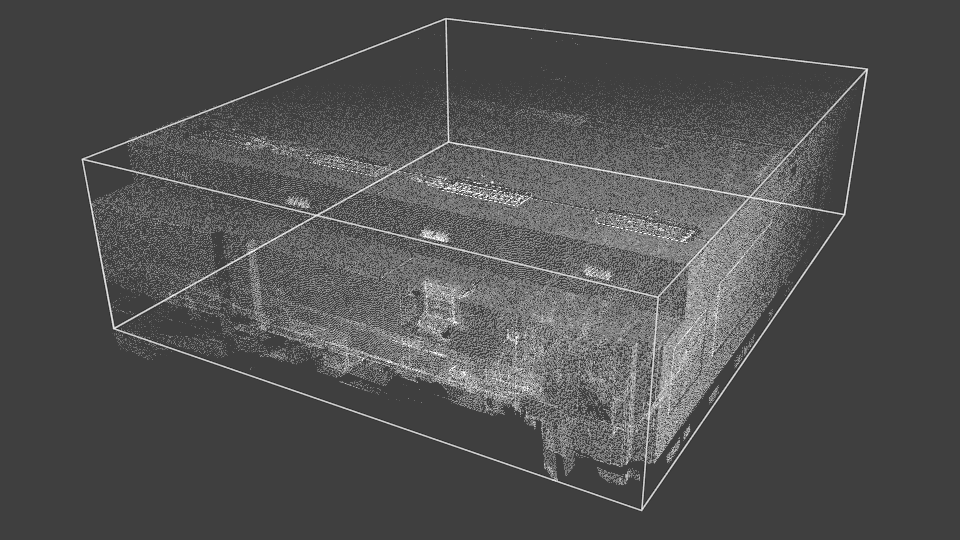
\includegraphics[width=1\linewidth]{Includes/images/Appendix/bound1}
\caption{Point Cloud With Boundaries Overlaid}
\label{fig:bound1}
\end{figure}
\begin{figure}[H]
\centering
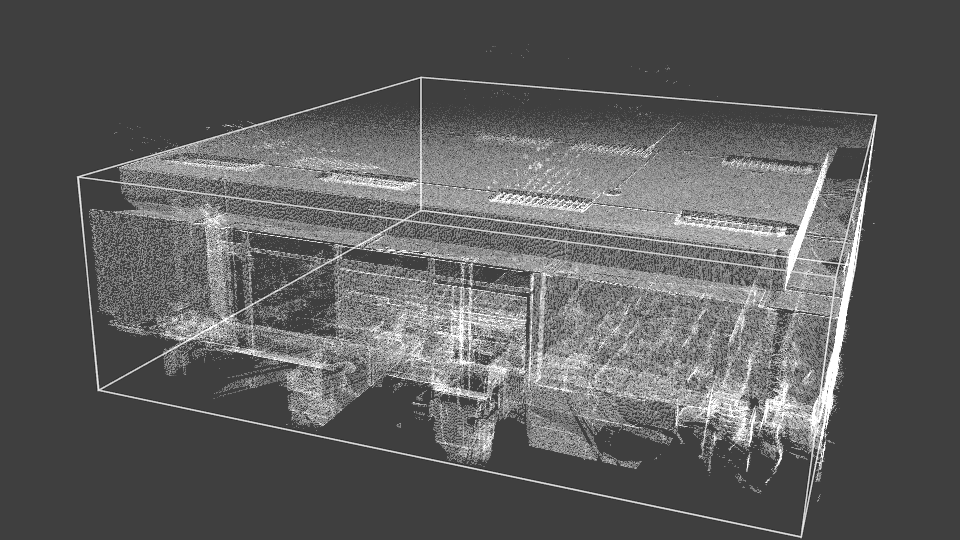
\includegraphics[width=1\linewidth]{Includes/images/Appendix/bound2}
\caption{Point Cloud With Boundaries Overlaid from a different angle}
\label{fig:bound2}
\end{figure}

All The Starting Point Clouds, Segmented Point Clouds and Final Boundary Representations have been submitted with this Report on a CD, along with all C++ Code.


